\section{Design Rationale}

\begin{figure*}[t!]
\centering
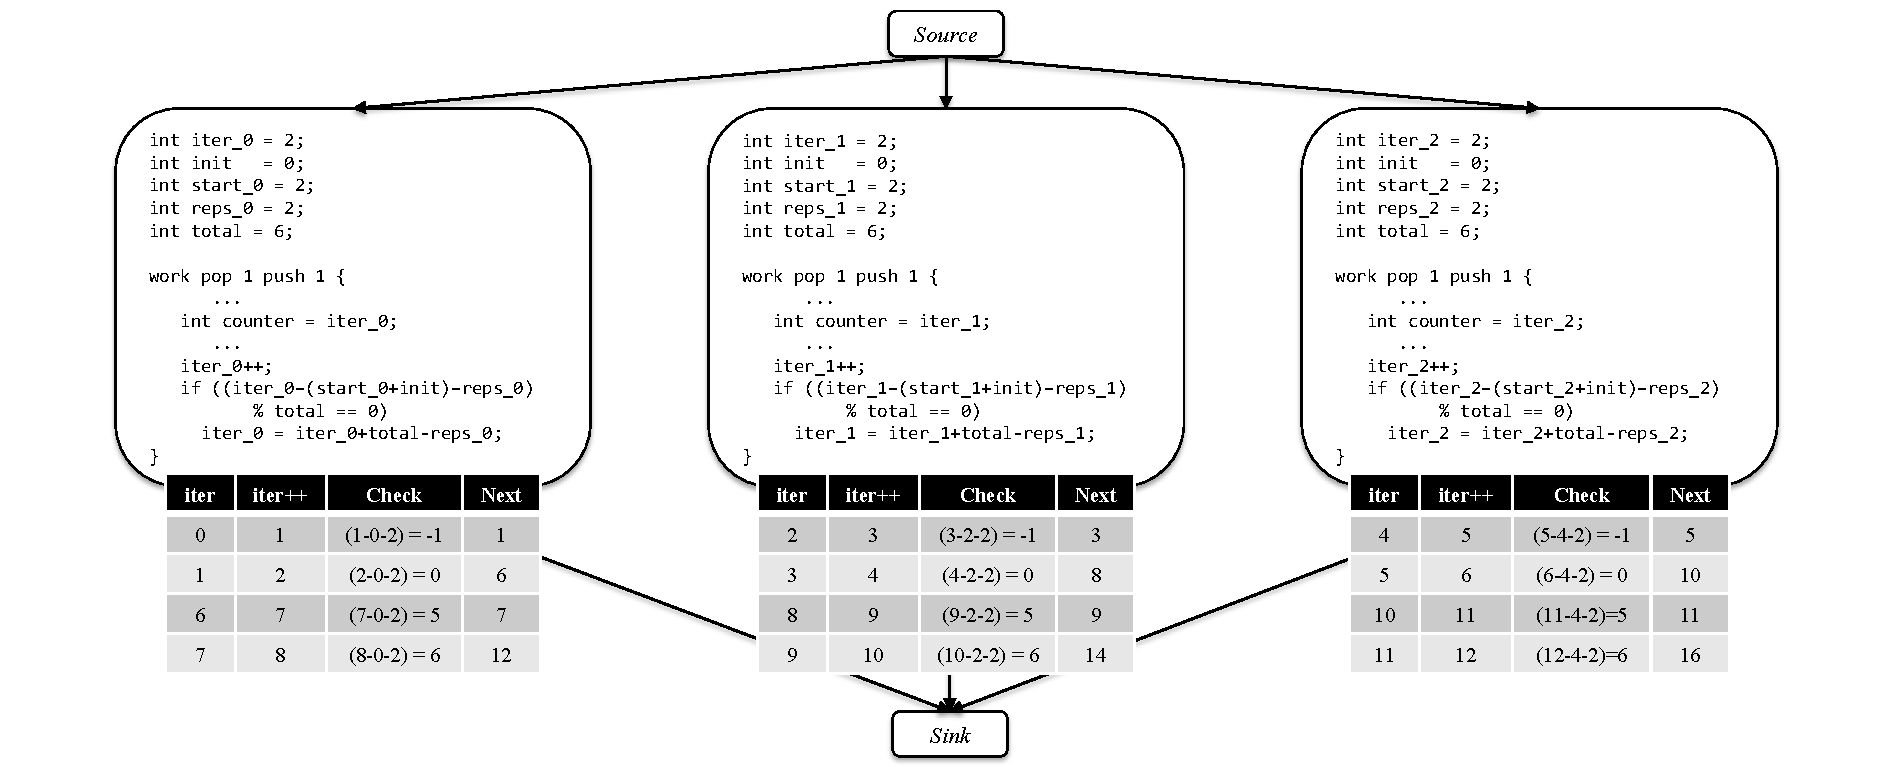
\includegraphics[width=6.5in]{figures/fission-example.pdf}
\caption{NEED CAPTION.\protect\label{fig:fission-example}}
\end{figure*}

Our approach in removing induction variable state is to introduce a new language construct.  The language construct maintains a value indicating how often the corresponding filter has been invoked.  This approach was chosen over implementing a system to automatically recognize induction variable usage in filter construction.

The approach of automatic analysis would require looking for an induction variable defined in the filter.  The simplest form of this analysis would require first idiomatically detecting for a variable modified by a statement similar to \texttt{var = var + 1}.  Very few iteration filters (outside of source filters) use induction state in this limited capacity.  Consider Figure~\ref{fig:weight-calc}, where the induction variable is incremented at each iteration step, until a certain threshold value at which it will reset.  This pattern is very common in programs that use induction filters.  MPD and FIRBank use this technique to iterate across a provided array one element per iteration step.  To ensure consistency between iteration steps, the automatic analysis is required to detect these types of updates as well.  

\begin{figure}[t]
{\eightpoint
\begin{verbatim}
float->float stateful filter WeightCalc(int n)
{
  float[n] window;
  int windowPos;

  ...

  // the input stream is multiplied with the weights
  work push 2 pop 2
  {

    push(pop() * window[windowPos]);
    push(pop() * window[windowPos]);

    windowPos++;
    if(windowPos >= n)
    {
      windowPos = 0;
    }
  }
}
\end{verbatim}
\caption{MPD filter that multiplies stream values with weights.\protect\label{fig:weight-calc}}}
\end{figure}

\begin{figure}[t]
{\eightpoint
\begin{verbatim}
float->float stateful filter CFARDetectFilter(int rows, int cols)
{
  int currentCol;
  int currentRow;

    ...

  work pop 3 push 1
  {
      ...

    currentRow++;
    if(currentRow >= rows)
    {
      currentRow = 0;

      currentCol++;
      if(currentCol >= cols)
      {
        currentCol = 0;
      }
    }
  }
}
\end{verbatim}
\caption{MPD CFAR Detect filter.\protect\label{fig:cfar-detect-filter}}}
\end{figure}

A filter may have multiple induction variables that are dependent on one another in defining their values.  Consider Figure~\ref{fig:cfar-detect-filter}, a filter used in MPD maintaining nested induction variables.  The automatic analysis must also be able to detect incrementing statements that may not necessarily be updated on every work call.  The process of simply detecting and identifying induction variables can potentially branch into many cases that need to be specially implemented.

There may potentially be other special cases that must be defined into the automatic analysis.  Filters may have also define induction variables to start with and reset to a particular value.  Induction variables may increment by a different value other than 1 at each execution step.  Though the methods of using induction variables as illustrated in Figure~\ref{fig:cfar-detect-filter} and Figure~\ref{fig:weight-calc} encompass many of the common use cases in the benchmark suite, slight variations in the implementation to the pattern may prevent the induction variable from being detected.

Accordingly, there are several downsides to the approach of automatic analysis.  Automatic recognition is a fairly inflexible process in detecting induction variable state.  As illustrated, there may be many different ways of defining induction variables.  Nested counters are often used to track row and column indexes in two-dimensional arrays.  Co-induction variables may be constructed to reset the value of other variables after reaching a certain value.  The many different uses of induction variables may be difficult to assess.  Automatic recognition would restrict data parallelism opportunities to only the filters that fit the implemented templates.  We instead elect to provide the user with the flexibility of defining derived induction values while providing parallelism opportunities.  

The keyword solution also has the added benefit of maintaining a value that is predictable in its updates.  The value that the keyword returns is simply the current iteration number for that the corresponding filter has run.  This is a value that always increments by one at the end of every work call.  Automatic recognition is a frail process because it is difficult to predict how the induction value will be updated, as illustrated in the above figures.  

The approach of automatic analysis also does little to encourage programming with parallelism in mind.  User written code will still maintain state, which inhibits data parallelism opportunities.  In introducing a language construct, user written code eliminates explicitly kept state.  This approach encourages users to write code with the intention of exploiting parallelism.


